\section{The Metropolis-Hastings Algorithm}

\textit{Metropolis-Hastings algorithm} is one of the most used \textit{Markov Chain Monte Carlo}(MCMC) algorithm.
The \textit{Metropolis algorithm} was first introduced by Nicholas Metropolis in 1953 in his paper entitled \textit{"Equation of State Calculations by Fast Computing Machines"}, with Arianna W. Rosenbluth, Marshall Rosenbluth, Augusta H. Teller and Edward Teller.
Arianna Rosenbluth wrote the first full implementation of Metropolis Algorithm for  \textit{Mathematical Analyzer Numerical Integrator and Automatic Computer Model I}(MANIAC 1) which was an early computer built under the direction of Nicholas Metropolis at the Los Alamos Scientific Laboratory.

\begin{figure}[H]
	\centering
	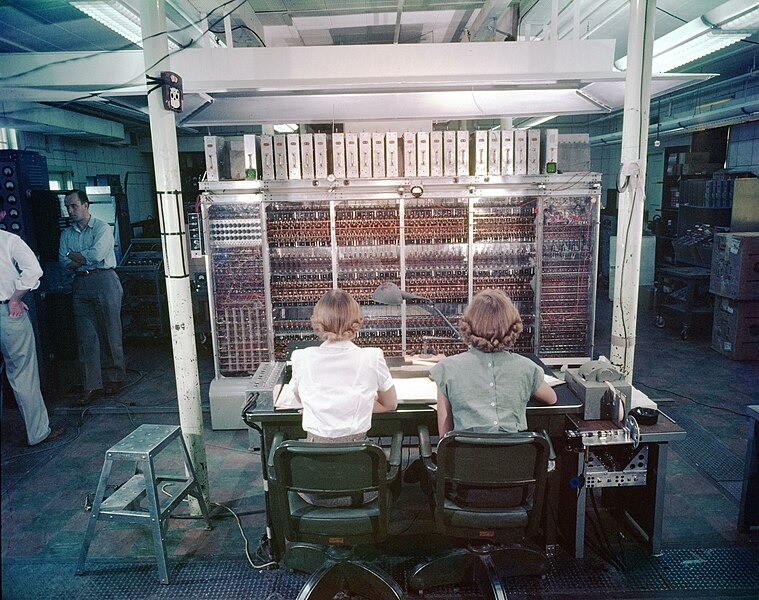
\includegraphics[width=0.4\textwidth]{Operators_in_front_of_the_MANIAC.jpg}
	\caption{MANIAC 1 one of the earliest computer.}
	\label{MANIAC}
\end{figure}

For may years this algorithm is was simply known as \textit{Metropolis Algorithm}, later in 1970 W.K. Hastings introduce more general version of this algorithm in his paper \textit{"Monte Carlo Sampling Methods Using Markov Chains and Their Applications"}. This generalized Metropolis algorithm is known as \textit{Metropolis-Hastings algorithm}(MH algorithm).

Suppose we want to simulate a random variables or sequence of random variable with probability mass function
\begin{equation}
	\pi(\theta) = \frac{f(\theta)}{K}
\end{equation}
where $ K $ is normalizing constant which is unknown or difficult to compute.

One way to simulate $ \pi(\theta) $ is to constant a Markov Chain that is easy to simulate and whose limiting distribution is $ \pi(\theta) $.
The \textit{Metropolis-Hastings algorithm} do exactly this. MH algorithm constant a time-reversible Markov Chain with desired limiting probabilities.

\subsection{Algorithm for Metropolis-Hastings}
\begin{enumerate}
	\item Start with any \textbf{initial state}  $ \theta_0 $ satisfying $ f(\theta) > 0 $.
	\item Using a \textbf{current state}  $ \theta $, sample \textbf{candidate state} $ \theta' $ for some \textbf{jumping distribution} $ q(\theta, \theta') = q(\theta'|\theta) $, which is the probability of jumping to $ \theta' $ provided the current state in $ \theta $.
	\item Given the candidate state $ \theta' $ calculate the \textbf{acceptance probability} $ \alpha(\theta,\theta') $ by,
	      \[
		      \alpha(\theta,\theta') =\min\left( \frac{\pi(\theta')q(\theta', \theta)}{\pi(\theta)q(\theta, \theta')}, 1\right) = \min\left( \frac{f(\theta')q(\theta', \theta)}{f(\theta)q(\theta, \theta')} , 1\right)
	      \]
      \item  Accept the candidate point with probability $ \alpha $.

\end{enumerate}
We can summarize the Metropolis-Hastings Algorithm as first computing,
\[ 
    \alpha(\theta_{t},\theta_{t+1}) = \min \left( \frac{f(\theta_{t+1})q(\theta_{t+1},\theta_t)}{ f(\theta_t) q(\theta_t,\theta_{t+1}) } \right)
\]
and then accepting the candidate point $ \theta_{t+1} $ with probability $ \alpha $. This generates a Markov Chain $ ( \theta_0,\theta_1,\ldots,\theta_t,\ldots ) $,
as the transition probabilities from $ \theta_t $ to $ \theta_{t+1} $ depends only on $ \theta_t $ and not on $ (\theta_0,\theta_1,\ldots,\theta_{t-1}) $.

\subsection{Metropolis-Hastings Algorithm as a Markov Chain}
To determine Metropolis-Hastings Sampling generates a Markov Chain whose stationary distribution is candidate distribution $ \pi(\theta) $ if the Metropolis-Hastings transition kernel,
\begin{equation}
    \label{transition-kernel}
    P(\theta_1\to \theta_2) = P(\theta_1,\theta_2) = q(\theta_1,\theta_2)\alpha(\theta_1,\theta_2) = q(\theta_1,\theta_2)\times \min\left( \frac{f(\theta')q(\theta', \theta)}{f(\theta)q(\theta, \theta')} , 1\right)
\end{equation}
 is time-reversible and satisfies 
 \[
         P(\theta_1, \theta_2) \pi(\theta_1) = P(\theta_2, \theta_1) \pi(\theta_2)
 \]
 or 
 \begin{equation}
     \label{balance-equatation}
     q(\theta_1,\theta_2)\alpha(\theta_1,\theta_2)\pi(\theta_1) = q(\theta_2,\theta_1)\alpha(\theta_2,\theta_1)\pi(\theta_2) \ \forall \theta_1, \theta_2
 \end{equation}

 For time-reversibility we choose jumping distribution $ q(\theta_1,\theta_2) $ to be irreducible and $ q(\theta_1,\theta_2) = q(\theta_2,\theta_1) $ and for \Cref{balance-equatation} we consider the cases.

\textbf{Case 1:} $ q(\theta_1,\theta_2)\pi(\theta_1) = q(\theta_1,\theta_2)\pi(\theta_1)$ 
Hence, $$ \alpha(\theta_1,\theta_2) = \alpha(\theta_1,\theta_2) = 1 $$
In this case \Cref{balance-equatation} will easily holds.

\textbf{Case 2:} $ q(\theta_1,\theta_2)\pi(\theta_1) > q(\theta_1,\theta_2)\pi(\theta_1)$.
Hence,
\[
    \alpha(\theta_1,\theta_2) = \frac{\pi(\theta_2)q(\theta_2,\theta_1)}{\pi(\theta_1)q(\theta_1,\theta_2)} \ \ \text{and} \ \ \alpha(\theta_2,\theta_1) = 1
\]
Then,

\begin{align*}
    P(\theta_1,\theta_2)\pi(\theta_1) &= q(\theta_1,\theta_2)\alpha(\theta_1,\theta_2) \pi(\theta_1) \\ 
    &= q(\theta_1,\theta_2) \frac{\pi(\theta_2)q(\theta_2,\theta_1)}{\pi(\theta_1)q(\theta_1,\theta_2)} \pi(\theta_1) \\
    &= q(\theta_2,\theta_1) \pi(\theta_1) = q(\theta_2,\theta_1) \alpha(\theta_2,\theta_1) \pi(\theta_1) \\ 
    &= P(\theta_2,\theta_1) \pi(\theta_2)
\end{align*}
Hence this case satisfies \Cref{balance-equatation}.

\textbf{Case 3:} $ q(\theta_1,\theta_2)\pi(\theta_1) < q(\theta_1,\theta_2)\pi(\theta_1)$
Hence,
\[
 \alpha(\theta_1,\theta_2) = 1  \ \ \text{and} \ \  \alpha(\theta_2,\theta_1) = \frac{\pi(\theta_1)q(\theta_1,\theta_2)}{\pi(\theta_2)q(\theta_2,\theta_1)} 
\]
Then,
\begin{align*}
    P(\theta_2,\theta_1)\pi(\theta_2) &= q(\theta_2,\theta_1)\alpha(\theta_2,\theta_1)\pi(\theta_2) \\ 
                                      &= q(\theta_2,\theta_1) \frac{\pi(\theta_1)q(\theta_1,\theta_2)}{\pi(\theta_2)q(\theta_2,\theta_1)} \pi(\theta_2) \\ 
                                      &= q(\theta_1,\theta_2) \pi(\theta_1) = q(\theta_1,\theta_2) \alpha(\theta_1,\theta_2) \pi(\theta_1) \\ 
                                      &=P(\theta_1,\theta_2) \pi(\theta_1)
\end{align*}
Hence also for this case \Cref{balance-equatation} is satisfied.

\subsection{Burn-In period}
A main problem with the successful implementation of Metropolis-Hastings Algorithm infect any for any MCMC Methods is number of steps until the chain approaches stationarity.
Typically the first $ 25\% $ samples are thrown out. These are called burn-in of a sample.

The name "burn-in" comes form electronics. Many electronics components fail quickly, those that don't are more reliable subset. So a burn-in is done at the factory to eliminate the worst.

There is no rule how may samples are choose as burn-in, this is vary difficult problem to answer. A poor choice of initial values and/or jumping distribution can greatly increase the requirement of burn-in time, this a hot research topic how do we choose an optimal starting point and jumping distribution. For simplicity, we choose starting value to be as close as center of the candidate distribution. 

\textbf{"Burn-in is only one method, and not a particularly good method, of finding a good starting point"}

A chain is said to be \textbf{poorly mixing} if it says in small regions of the parameter
space for long periods of time, as opposed to a well \textbf{mixing chain} that seems to
happily explore the space. A poorly mixing chain can arise because the target
distribution is multimodal and our choice of starting values traps us near one of the modes. 
To avoid this issue we can use multiple highly dispersed initial values to start several different chains.

\subsection{Choosing Jumping Distribution}
Now the question arise how to choose a best jumping distribution that works? 
There are two approaches. First and must common one is the new value $ \theta_{t+1} $ equals the current value $ \theta_t $ plus a random noise $ z $. That is,
\[
    \theta_{t+1} = \theta_t + z
\]
In this case, $ q(\theta_{t},\theta_{t+1}) = g(\Theta_{t+1}-\theta_t) = g(z) $, the density associated with the random noise $ z $. If $ g(z) = g(-z) $, i.e., the density for the random variable $ z $ is symmetric.

Typically we take, $ z $ to be from normal or multivariate normal distribution with mean zero. Then, $ \theta_{t+1} $ is form normal or multivariate normal distribution with mean $ \theta_t $. 

Then, we can use Metropolis-Hastings sampling as,
\[
    \frac{q(\theta_t,\theta_{t+1})\pi(\theta_t)}{q(\theta_{t+1},\theta_{t})\pi(\theta_{t+1})}  = \frac{g(z)\pi(\theta_t)}{g(-z)\pi(\theta_{t+1})} = \frac{\pi(\theta_t)}{\pi(\theta_{t+1})}
\]
We can adjust the variance of jumping distribution to get better mixing.

Second one is, we use an independent chain. The probability of jumping to a point $ \theta_{t+1} $ is independent of current position $ \theta_t $ of the chain, i.e. $ q(\theta_t,\theta_{t+1}) = g(y) $. Thus the current value is simply drawn from a distribution of interest, independent of current position.

\subsection{Convergence Diagnostics}
Now we have to ensure that Markov Chains have reached stationarity and only use those samples that have been generated after stationarity has been reached. But it is impossible to ensure when those two conditions are satisfied since the Markov Chain does not begin with stationary distribution. Instead we can use various methods to assess whether or not stationarity appears to have reached. Most common one is:

\textbf{Visual inspection} where we plot variable of interest vs iteration number, plot running means of variables of interest etc or run various iteration of samples with different initial states and different jumping distribution and compare them. This method is manual and need lot of works.

Another one is \textbf{Geweke test}, splits sample (after burn-in period) into two parts.
Say the first 10\% and last 50\%. If the chain is at stationarity, the means of two samples should be equal. A modified z-test can be used to comparer the two subsamples,
and the resulting test statistic is often referred to as a \textbf{Geweke z-score}.
A value larger than 2 indicates that the mean of
the series is still drifting, and a longer burn-in is required before monitoring the
chain (to extract a sampler) can begin. Formula for Geweke z-score is given by,
\[
    z = \frac{\Bar{X_1} - \Bar{X_2}}{\sqrt{ \text{Var}(X_1) + \text{Var}(X_2) }}
\]
Where, $ X_1 $ is the first 10\% subsamples and $ X_2 $ last 50\% subsamples.

\subsection{Examples}

Now we see some examples how we can use Metropolis-Hastings Algorithm. 

\begin{example}[Simulating from an unknown distribution]
    The besis problem Metropolis-Hastings algorithm solves is to provided a method for sampling from some arbitrary probability distribution. In this example we see how it is works,

    Suppose, we have 
    \[
        p(x) = \frac{e^{(-x^2)} \left( 2 + \sin(5x) + \sin(2x) \right) }{ \int_{-\infty}^{\infty} e^{(-u^2)} \left( 2 + \sin(5u) + \sin(2u) \right) du }
    \]
    Now we want to generate a random variables form $ p(x) $. It is may very hard to calculate the integration in the denominator or we don't want to calculate it. i.e., we the the probability distribution up to normalizing constant.
    So we have,
    \[
        p(x) \propto e^{(-x^2)} \left( 2 + \sin(5x) + \sin(2x) \right) 
    \]
    \begin{figure}[H]
        \centering
        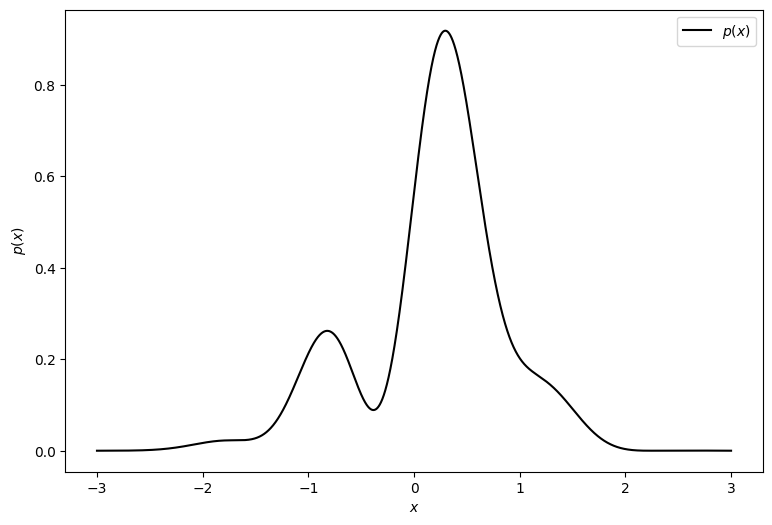
\includegraphics[width=0.6\textwidth]{./images/metropolis/plot-of-px.png}
        \caption{Plot of original $p(x)$}
        \label{plot of px}
    \end{figure}
    
\end{example}





